\subsubsection{Pengujian LED Blink pada RaspberryPi}

Pengujian sistem ini mencakup pengujian dengan ID P20, P21, P22, P23, P24, P25, P26, P27, P28, P29, P30 dan P31. Pada pengujian sistem ini, dilakukan proses \textit{remote deployment} untuk menyalakan lampu blink pada RaspberryPi dengan cluster "cluster-raspi". Dibuat sebuah script python yang berinteraksi dengan GPIO pada pin 2 untuk menyalakan lampu LED. Script dapat dilihat pada lampiran \ref{fig:raspi-python-led-script}

\begin{figure}[ht]
  \centering
  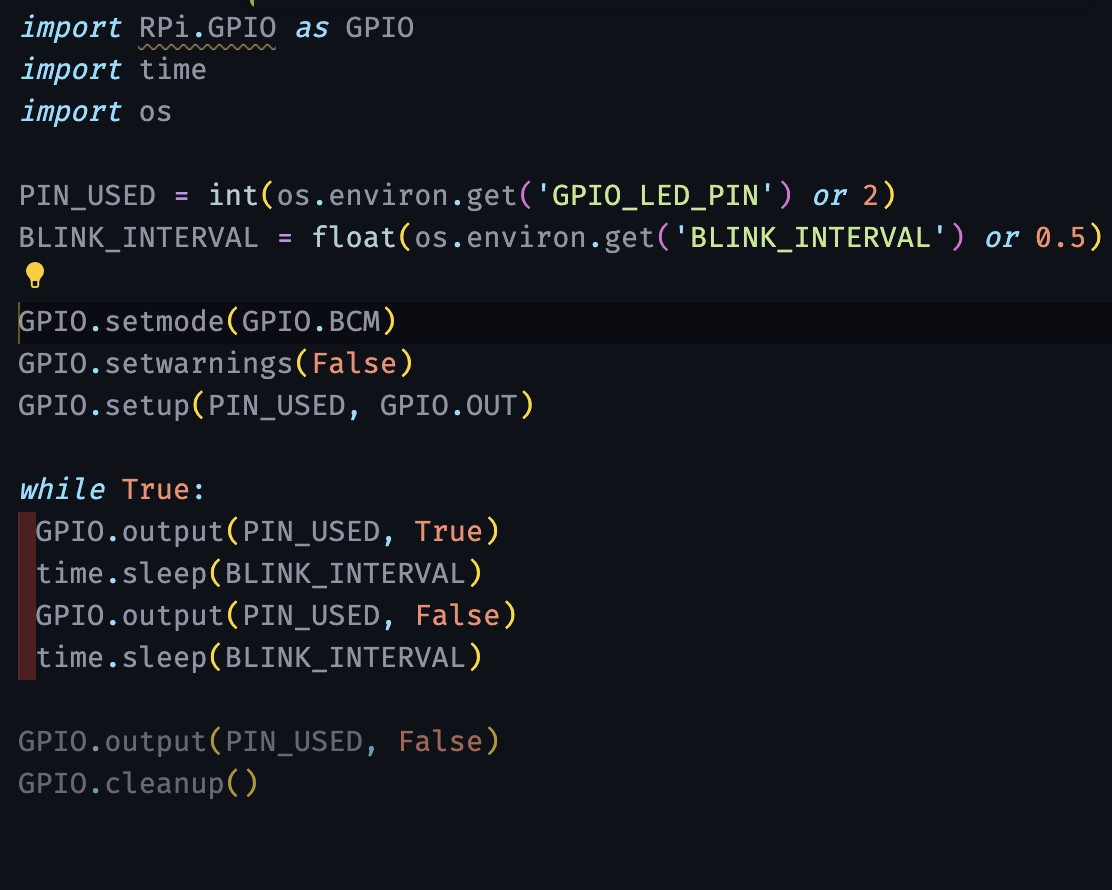
\includegraphics[width=0.8\textwidth]{resources/chapter-4/pengujian/pengujian-sistem-raspi-09-led.jpg}
  \caption{Python Raspi LED Script}
  \label{fig:raspi-python-led-script}
\end{figure}

Dari script tersebut, dibuat docker image dengan base image armv7 yang membungkus python tersebut agar dapat berjalan di sistem IoT. Docker image yang telah dibuat diunggah ke dockerhub dengan nama {gawrgare/led\textunderscore blink}. Isi dari dockerfile dapat dilihat pada lampiran \ref{fig:raspi-docker-led-script}. Setelah docker image tersedia, selanjutnya terdapat beberapa langkah yang harus disiapkan sebelum melakukan \textit{deployment} pada lingkungan raspberrypi.

\begin{enumerate}
  \item Membuat \textit{company} dengan nama "raspi-company" dan \textit{cluster\textunderscore name} "cluster-raspi". Hasil dapat dilihat pada lampiran \ref{fig:pengujian-sistem-raspi-01}
  \item Membuat user pada \textit{company} tersebut dengan email \textit{raspi@gmail.com}. Hasil dapat dilihat pada lampiran \ref{fig:pengujian-sistem-raspi-02}
  \item Login dengan kredensial yang telah dibuat
  \item Mengunjungi halaman /devices dan melakukan registrasi \textit{devices} untuk kedua RaspberryPi dengan daftar nama nodes yang dapat dilihat pada lampiran \ref{fig:pengujian-sistem-raspi-04}
        \begin{enumerate}
          \item \textit{Device} "raspi-master" untuk \textit{hostname masterpi} dengan nama \textit{cluster} yaitu "master-node-raspi"
          \item  \textit{Device} "raspi-worker" untuk \textit{hostname raspberrypi} dengan nama \textit{cluster} yaitu "worker-node-raspi"
        \end{enumerate}
  \item Mengunjungi halaman /groups dan membuat \textit{group} "raspi-group-blink". Hasil dapat dilihat pada lampiran \ref{fig:pengujian-sistem-raspi-05}
  \item Mengunjungi halaman group detail "raspi-group-blink" lalu menambahkan kedua device ke dalam group.
  \item Mengunjungi halaman \textit{deployment} lalu membuat repository dengan nama "raspi-image-blink" dan image\textit{ gawrgare/led\textunderscore blink}.
  \item Membuat deployment dengan nama "raspi-deployment-blink" dan mengisi target dengan "node=master" pada halaman \textit{deployment}.
\end{enumerate}

Layout dari RaspberryPi serta letak kabel dan LED dapat dilihat pada lampiran \ref{fig:pengujian-sistem-raspi-layout}. Setelah semua persiapan dilakukan, dilakukan pengujian dengan dua jenis \textit{deployment} yaitu \textit{target} dan \textit{custom} dengan versi \textit{group}.
\begin{enumerate}
  \item Target deployment merupakan deployment yang dilakukan sesuai dengan nilai target pada deployment object, dalam kasus ini target nya ialah node dengan attribut "node=master". Pengujian tipe ini hanya melakukan deployment dengan \textit{hostname masterpi} yang memiliki nama node "master-node-raspi". Setelah deployment dilakukan, LED yang terhubung dengan pin pada "master-node-raspi" berkedip, hal ini menunjukan bahwa proses deployment telah berhasil dilakukan. Hasil dapat dilihat pada lampiran \ref{fig:hasil-pengujian-sistem-raspi-target}.
  \item Custom deployment mengabaikan nilai target yang terdapat pada objek deployment dan melakukan deployment sesuai jenis serta id yang diinginkan. Terdapat dua jenis yaitu \textit{group} dan \textit{device}. Dalam kasus groups, Deployment dilakukan ke dua \textit{device} yang terhubung ke \textit{group} "raspi-group-blink". Setelah deployment dilakukan, kedua LED berkedip menunjukan bahwa script berhasil dijalankan untuk setiap \textit{device} yang terhubung pada group. Hasil dapat dilihat pada lampiran \ref{fig:hasil-pengujian-sistem-raspi-custom}.
\end{enumerate}

Setelah deployment berhasil dilakukan, pengujian dilanjutkan dengan mengunjungi halaman detail dari "raspi-deployment-blink" untuk melihat riwayat deployment. Hasil dapat dilhat pada lampiran \ref{fig:pengujian-sistem-raspi-10}. Dapat dilihat bahwa pengujian dengan ID P20 hingga P31 menunjukan hasil yang sesuai dengan kebutuhan fungsional yang telah didefinisikan. Seluruh rekap pengujian sistem ini dapat dilihat pada lampiran \ref{tab:pengujian-sistem-raspi}.